\section{Results}
The baseline comparison completed all 99 cases. The first profile pass completed
297 of 300 jobs; a separate documented retry recovered the three failed
original-model conductance profiles. Both passes are retained. None of the
completed profiles found a minimum requiring a baseline refit under the recorded
tolerance. The bootstrap completed all 96,000 planned refits, and the working
OU likelihood comparison completed all 48 calibrations. Independent synthetic
coverage and prospective-design results remain in progress.

\subsection{Order and initialization}
The startup assumption reverses the order ranking for the sine and joint
calibrations (Fig.~\ref{fig:baseline-order}). For these two calibration sets,
cold delay states give the lowest error at one stage among the compared
formulations. Equilibrated states favor
the pure-delay limit. The step experiment with equilibrated states gives the
same error for every order, as expected from the delay's absence from its
response. These comparisons concern calibration error under prescribed histories;
they do not establish which history occurred before recording began.
Table~\ref{tab:calibration-rmse} gives the numerical comparison, including the
step calibration, where the cold two-stage model improves on the cold one-stage
fit. Table~\ref{tab:joint-parameters} gives the joint cold parameters.
% Generated by render_tables.py; edit the producer, not this table.
\begin{table}[tbp]
\centering
\small
\begin{tabular}{lrrrr}
\toprule
Model & Sine, cold & Step, cold & Joint, cold & Joint, equilibrated \\
\midrule
$n=1$ & 0.2567 & 0.1573 & 0.4115 & 0.7936 \\
$n=2$ & 0.3470 & 0.1529 & 0.4630 & 0.7585 \\
$n=3$ & 0.3810 & 0.1573 & 0.4841 & 0.7486 \\
$n=4$ & 0.3985 & 0.1610 & 0.4953 & 0.7441 \\
$n=6$ & 0.4165 & 0.1659 & 0.5070 & 0.7398 \\
$n=8$ & 0.4256 & 0.1689 & 0.5130 & 0.7378 \\
$n=12$ & 0.4348 & 0.1724 & 0.5192 & 0.7359 \\
Pure delay & 0.4541 & 0.1812 & 0.5323 & 0.7322 \\
\bottomrule
\end{tabular}
\caption{Calibration RMSE in degrees Celsius, excluding the initial temperature. Each entry comes from its own fitted calibration/startup combination. Equilibrated means the prescribed delay states equal the initial command, with the sensor temperature fixed by the first observation.}
\label{tab:calibration-rmse}
\end{table}

% Generated by render_tables.py; edit the producer, not this table.
\begin{table}[tbp]
\centering
\small
\begin{tabular}{lrrrrr}
\toprule
Model & $K$ & $\tau$ (s) & $\theta$ (s) & $\Ua$ (W/K) & $\Cp$ (J/K) \\
\midrule
$n=1$ & 0.7744 & 150.697 & 16.555 & 0.04132 & 6.227 \\
$n=2$ & 0.7762 & 154.197 & 15.403 & 0.04123 & 6.357 \\
$n=3$ & 0.7768 & 155.291 & 15.074 & 0.04119 & 6.397 \\
$n=4$ & 0.7771 & 155.826 & 14.917 & 0.04118 & 6.417 \\
$n=6$ & 0.7774 & 156.353 & 14.764 & 0.04116 & 6.436 \\
$n=8$ & 0.7776 & 156.614 & 14.689 & 0.04115 & 6.445 \\
$n=12$ & 0.7777 & 156.874 & 14.614 & 0.04115 & 6.455 \\
Pure delay & 0.7780 & 157.391 & 14.466 & 0.04113 & 6.474 \\
\bottomrule
\end{tabular}
\caption{Joint cold-start estimates. Gain units are degrees Celsius per percentage-point command. Physical columns transform the IO estimates using fixed $c=0.032$ W per percentage point; they are effective-model quantities. The one-stage row uses the representative $\tau\geq\theta$.}
\label{tab:joint-parameters}
\end{table}


\begin{figure}[p]
 \centering
 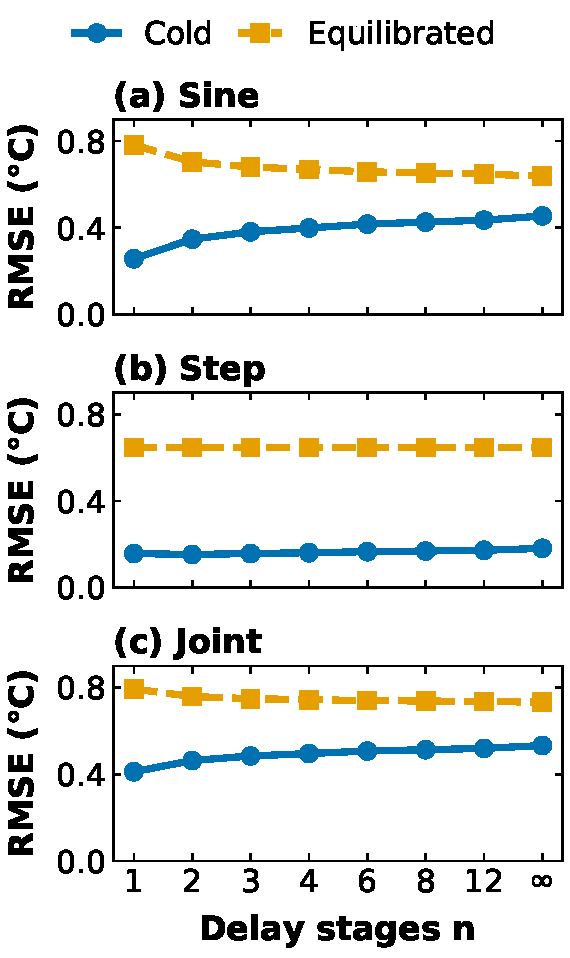
\includegraphics[width=.5\linewidth]{baseline_order.pdf}
 \caption{Initialization changes the fitted order ranking. Root mean squared
 temperature error (RMSE) for sine, step, and joint calibration is plotted for
 input--output parameter fits. Cold means $z_i(0)=0$; equilibrated means
 $z_i(0)=u(0)$. The infinity label denotes the separately fitted pure-delay model,
 with the corresponding input prehistory. Lines connect categorical orders as
 guides. Every error excludes the first temperature used to initialize the
 model. No uncertainty intervals are implied by the markers.}
 \label{fig:baseline-order}
\end{figure}

\subsection{Temperature traces and residuals}
The jointly calibrated cold models give closely spaced temperature predictions,
while their residual traces show differences near startup and the sine peaks
(Fig.~\ref{fig:baseline-trajectories}). Residual structure persists over many
successive observations. A visual match on the full temperature scale therefore
does not establish independent sensor noise or reliable uncertainty coverage.

\begin{figure}[p]
 \centering
 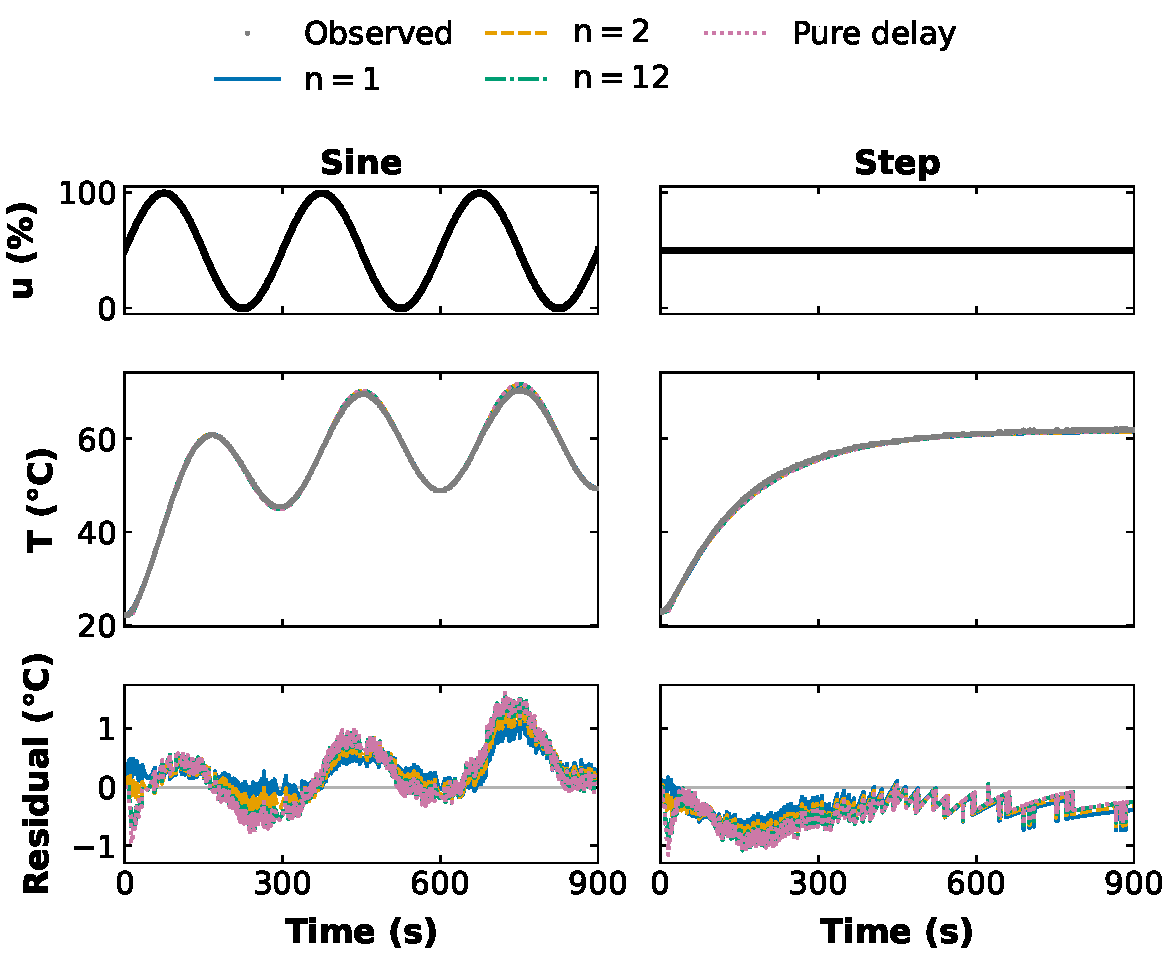
\includegraphics[width=\linewidth]{baseline_trajectories.pdf}
 \caption{The residual scale exposes differences hidden in the temperature
 overlays. Columns show the sine and step experiments; rows show heater input
 $u$, measured temperature $T$ with jointly fitted cold-start mean predictions,
 and residuals defined as prediction minus observation. All recorded calibration
 samples are plotted. The thermal initial condition and assumed ambient equal
 the first observation, and the delay prehistory is zero. The four curves use
 independent joint fits for their respective formulations. These are mean
 predictions; uncertainty bands are not shown.}
 \label{fig:baseline-trajectories}
\end{figure}

\subsection{Coordinate conditioning and physical ambiguity}
The independently fitted physical and input--output formulations reach sums of
squares that agree to numerical precision in the joint cold cases
(Table~\ref{tab:coordinate-metrics}). Reexpressing the same sensitivity matrix
changes its condition number. Moment coordinates do not improve this particular
metric at these fitted points. These differences concern the coordinate metric;
they do not distinguish observationally equivalent model explanations.
% Generated by render_tables.py; edit the producer, not this table.
\begin{table}[tbp]
\centering
\small
\begin{tabular}{lrrrr}
\toprule
Model & IO logs & Physical logs & Moment & $|\Delta S|$ \\
\midrule
$n=1$ & 23.1 & 19.38 & 27.76 & $6.3\times10^{-12}$ \\
$n=2$ & 21.04 & 17.56 & 24.82 & $1.5\times10^{-11}$ \\
$n=3$ & 20.61 & 17.19 & 24.15 & $1.3\times10^{-12}$ \\
$n=4$ & 20.44 & 17.04 & 23.86 & $4.3\times10^{-11}$ \\
$n=6$ & 20.29 & 16.9 & 23.6 & $2.1\times10^{-11}$ \\
$n=8$ & 20.23 & 16.84 & 23.48 & $3.2\times10^{-12}$ \\
$n=12$ & 20.16 & 16.78 & 23.36 & $3.4\times10^{-13}$ \\
Pure delay & 20 & 16.64 & 23.09 & $8.0\times10^{-11}$ \\
\bottomrule
\end{tabular}
\caption{Coordinate metrics for joint cold fits. The first three columns are sensitivity condition numbers at the same IO model point, transforming the information matrix without refitting. Moment coordinates are $(\log K,\log m,\ell)$ with $m=\tau+\theta$ and $\ell=\log[\theta/\tau]$. The last column compares independently fitted IO and physical sums of squares, in squared degrees Celsius. Conditioning changes do not imply additional information.}
\label{tab:coordinate-metrics}
\end{table}


The original model has a stronger ambiguity. For each calibration, the saved
structural calculation sampled 403 positive physical parameter combinations with
the same transfer function. Their largest prediction difference was below
$1.8\times10^{-12}\,{}^\circ\mathrm C$. Conductance $\Ua$ remained fixed while
$\Ub$, $\CpH$ and $\CpS$ varied. Appendix~\ref{sec:structural} gives the
analytic family and its positivity limits; sampled ranges are not confidence
intervals.

The analytic family also exposed an interpolation failure. All nine redundant
physical-parameter profiles excluded some known equivalent family members from
their interpolated 95\% grid sets. The sampled objective values along the flat
region were correct; coarse interpolation across its rising edge produced the
misleading endpoints. We therefore withhold those endpoints as physical
confidence claims. The merged profile catalog records this finding separately
from the successful likelihood arithmetic and nuisance-fit checks. A converged
pointwise optimizer and a plotted crossing do not validate the whole profile set.

\subsection{Conditional delay uncertainty}
Table~\ref{tab:delay-uncertainty} compares delay uncertainty for representative
joint cold formulations. Increasing the residual block length widens the
percentile intervals relative to independent Gaussian simulation. The one-stage
profile has two accepted pole-label modes; canonical bootstrap summaries refer
to only the representative with $\tau\geq\theta$. A finite full-coordinate
interval is withheld where the recorded experiment leaves delay unobservable.
The table compares assumptions rather than estimating a single unconditional
physical uncertainty.
% Generated by render_tables.py; edit the producer, not this table.
\begin{table}[tbp]
\centering
\small
\begin{tabular}{lcccc}
\toprule
Model & IID profile set & IID simulation & Circular block 60 & OU local SD \\
\midrule
$n=1$ & $[16.35,16.76]\cup[150.2,151.2]$ & $[16.44,16.69]$ & $[15.62,17.56]$ & 0.585 \\
$n=2$ & $[15.2,15.6]$ & $[15.3,15.51]$ & $[14.31,16.44]$ & 0.606 \\
$n=12$ & $[14.41,14.82]$ & $[14.52,14.72]$ & $[13.25,15.98]$ & 0.654 \\
Pure delay & $[14.26,14.67]$ & $[14.38,14.56]$ & $[13.34,15.68]$ & 0.317 \\
\bottomrule
\end{tabular}
\caption{Joint cold delay uncertainty in seconds. Profile sets use a profiled common IID variance and retain both one-stage pole modes. Percentile intervals use 400 Gaussian simulations at fixed $\sigma=0.25$ degrees Celsius or 400 circular residual-block refits, respectively. Bootstrap one-stage delays use the canonical pole representative. OU entries are local standard deviations with variance profiled and length included in the Hessian, not interval endpoints. These procedures make different assumptions and are not interchangeable coverage guarantees.}
\label{tab:delay-uncertainty}
\end{table}


\subsection{The working correlated-noise model remains inadequate}
The independent innovations audit reproduced every saved OU likelihood within
$2.6\times10^{-12}$. This validates likelihood arithmetic, not the residual
model. Filtered innovations retain strong negative lag-one correlation
(Table~\ref{tab:ou-diagnostics}). The fitted length therefore cannot be treated
as a measured thermal disturbance time scale. Mean prediction errors on the
held-out records also remain much larger than calibration errors. Allowing
serial covariance changes conditional uncertainty without establishing that
the thermal mean transfers between records.
% Generated by render_tables.py; edit the producer, not this table.
\begin{table}[tbp]
\centering
\small
\begin{tabular}{lrrrr}
\toprule
Model & Length (s) & $\hat\sigma$ (${}^\circ$C) & ACF1, sine & ACF1, step \\
\midrule
$n=1$ & 17.46 & 0.4088 & -0.5333 & -0.492 \\
$n=2$ & 22.14 & 0.459 & -0.5291 & -0.4935 \\
$n=12$ & 27.91 & 0.5151 & -0.5253 & -0.4877 \\
Pure delay & 29.33 & 0.5289 & -0.518 & -0.4811 \\
\bottomrule
\end{tabular}
\caption{Working OU fits to the two joint cold records. The scale is the maximum-likelihood stationary residual standard deviation. ACF1 is the centered sample lag-one correlation of filtered innovations. Strong remaining negative correlation challenges this one-component residual covariance; a high fitted likelihood does not validate it.}
\label{tab:ou-diagnostics}
\end{table}


The remaining empirical results will be inserted after the independent coverage,
ambient/history sensitivity, validation and prospective-design audits finish.
\FloatBarrier
